% vim:ft=tex
\section{The model}
\label{sec:the-model}
%	There should be an introduction here. What will the reader learn during the section. 	%

\subsection{Social force models}
The idea behind social force models is that each individual in the crowd acts on his/ her own from a personal aim or goal and by behavioral reactions to
the environment. Different forces such as other pedestrians, walls and obstacles are taken into account when pedestrian $\alpha$ walks toward his/her aim or
goal, so that $\alpha$ does not walk into another pedestrian or wall. The forces influencing the pedestrian $\alpha$'s motion of direction are not forces
acting on $\alpha$'s body, but has to be seen as a quantity that describes the motivation to act.
Since pedestrian $\alpha$ is used to the situations he/she is normally confronted with, his/her reactions will be rather automatic and determined by his/her
experience of which reaction will be that best. Since the reaction is rather automatic it is possible to put the rules of pedestrian behavior into an
equation of motion. [Helbing and Molnár, 1995]

There are other ways to model crowd than social force models such as Rule Based models, Cellular Automata models and HiDAC. Below we will make a short
explanation of each of the other crowd models.
\\

\textbf{Rule Based models}\\
Rule Based models describe the movement of pedestrians through sets of basic rules. Each pedestrian apply collision detection and avoidance to prevent
collision with other pedestrians. However they do not in general apply collision response, and therefore collisions and overlappping of the pedestrians
may occur under some circumstances. Some models have applied stopping rules to prevent these situations. [Pelechano et al., 2008]

\textbf{Cellular Autamata models}\\
These models are discrete, deterministic and is made up of cells like the squares in a chessboard.
An artificial intelligence approach is used in Celluar Automata (CA) defined as mathematical idealisation of physical systems in which time and space are
discrete, and physical quantities take a finite set of discrete values. Pedestrian can not collide since the floor is dicretised and the pedestrians can
only move to free adjecent cells. [Pelechano et al., 2008]

\textbf{HiDAC}\\
The HiDAC model is made as a hybrid between social force models and rule based models. The motion of the pedestrians is caried out like the social force
models, but is also based on the psychological and geometrical rules. It peforms collision detection and response and rules are applied depending on the
pedestrian's personality and the state of the environment. [Pelechano et al., 2008]
\\
\\

\textbf{Geometrical features of the models}\\
Each of the different models have some geomatrical features relatively important and unimportant according to our simulation.

\textbf{Shaking} Wether pedestrians appear to shake when simulating the model.
When simulating the social force models the pedestrians seems to shake when cloggings and queues arise. This is caused by the modification
of each pedestrians postition in each timestep. 
The HiDAC, CA and rule based model do not appear to shake while the simulation run.

\textbf{Discrete and Continuous movement} Wether the space and time are discretised. In the CA model the pedestrians move between discritised adjecent
cells in one time step, and therefore have limited direction to go. The other models do not discretise space and therefore allow the pedestrians to move
within continuous space.
 
\textbf{Overlapping} Wether overlapping of the pedestrians is possible. The rule based models and the CA models do have collision detection but not
all have collision responce. The CA models have rules so that a pedestrian can not walk into an occupied cell, but if two pedestrians want to pass each
other they step into the cell diagonal to their own cell, and in their way cross the other pedestrian in the intersection between the four cells.
Newer models of the rule based and CA have made a stopping rule so that overlapping can not accour. The HiDAC and social force models do collision responce
to minize the risk of overlapping. [Pelechano et al., 2008]

\textbf{Pushing} Wether pedestrians can have physical contact. If the pedestrians can have physical contact they will be able to push each other in some
direction. This ability is possible when using the HiDAC and the social force model. When simulating evacuations and chaotic events it has been observed
that people do have physical contact and push each other [Helbing et at., 2005].

\textbf{Communication} Wether the pedestrians can share information about he environment. The HiDAC and som newer rule based models allows the pedestrians
to share information about the environment and to give orders. This feature is not included in social force models and CA. [Pelechano et al., 2008]

To illustrate different features of the different models the table below sums up the above mentioned.
\begin{center}
\begin{tabular}{lllll}
 & Social Forces & Rule Based & CA & HiDAC\\
Shaking avoidance     & - & + & + & +\\
Continuous space      & + & + & - & +\\
Overlapping avoidance & + & * & - & +\\
Pushing               & + & - & - & +\\
Communication         & - & * & - & +
\end{tabular}
\end{center}
Here ``+`` indicates that the feature is possible, ``-`` indicates it is not, and ''*'' that the model has been adjusted such that the feature have
become possible. [Pelechano et al., 2008]

The features we are interested in and find relevant in our simulation are continuous space, pushing and overlapping avoidance. The continuous space is
relevant for our simulaion to be as realistic as possible since we do not want our pedestrians to have at most nine directions to go each timestep.
The feature of pushing is also important to include since in panic sitiation it has been seen that people push each. This feature will then make our
simulation more realistic.
The overlapping avoidance we find relevant since this enables pedestrians to walk through each other.


\subsection{Explanation of our model}

%	I think we should add that this section is meerly a walk through the model and that		%
%	the different parts of the model will be discussed in a later section so the reader		%
%	wont feel that we leave out a lot of detail.											% 

In this section we will go through the model from the article \cite{self-org} in great detail. 
First of all,  as stated briefly earlier this model is an agent based social force model. 
This means that the model uses individual entities to say something about the crowd as a whole. 
Each entity or agent is acted on by a collection of different forces. These forces can be
either repulsive or attractive. The general approach of the model is fairly simple. An agent
$\alpha$ wants to go in a desired direction with a desired speed. However the environment 
and other agents might force agent $\alpha$ to stray from the desired direction or have speeds 
different from the desired one. The change in position of agent $\alpha$ is given by:

	\begin{equation}
		\frac{d \vec{r_{\alpha}}}{dt} = \vec{V_{\alpha}} \left( t \right)
	\end{equation}

And, as we know from newtonian physics, the acceleration of agent $\alpha$ is 
then given by the summation of all the forces acting on the agent:

\begin{equation}
    \frac{d \vec{V_{\alpha}}}{dt} = \vec{f_{\alpha}} \left( t \right) + 
    \vec{\xi_{\alpha}}\left( t \right)
\end{equation}

here $\vec{\xi_{\alpha}} \left( t \right)$ is a random fluctuation of agent $\alpha$. This
force is there to incorporate the fact that fact the identical initial condition
generally will not lead to the same series of events. $\vec{f_{\alpha}} \left( t \right)$ 
is a summation of all the forces action in agent $\alpha$ from the environment 
and other agents. More specifically it is given by:

\begin{equation}\label{model}
    \vec{f_{\alpha}} = \vec{f^{0}_{\alpha}}\left( \vec{V_{\alpha}} \right) + 
    \vec{f_{\alpha B}} \left( \vec{r_{\alpha}} \right) +
    \sum_{\beta \neq \alpha} \vec{f_{\alpha \beta}} \left(\vec{r_{\alpha}}, 
    \vec{V_{\alpha}}, \vec{r_{\beta}}, \vec{V_{\beta}} \right) +
    \sum_{i} \vec{f_{\alpha i}} \left( \vec{r_{\alpha}}, \vec{r_{i}}, t 
    \right)
\end{equation}

So this is a summation of four different kinds of forces. We will go through 
them one at a time explaining their role in the model and their mathematical 
structure. The first term on the right hand side is a velocity dependent force 
and it is given by:

\begin{equation}
	\vec{f^{0}_{\alpha}}\left( \vec{V_{\alpha}} \right) =
    \frac{1}{\tau}
    \left( V_{\alpha}^{0} \vec{e_{\alpha}} - \vec{V_{\alpha}} \right)
\end{equation}

Here $\tau$ is the relaxation time. $\vec{V_{\alpha}}$ is the 
current velocity of the agent and $V_{\alpha}^{0}$ is the initial speed, that is 
the speed of the agent at the end of the last simulation step. $V_{\alpha}^{0}$ is given by:

\begin{equation}
    V_{\alpha}^{0} = \left[ 1 - \eta_{\alpha} \left( t \right) \right] 
    V_{\alpha}^{0} \left( 0 \right) +
    \eta_{\alpha} \left( t \right)V_{\alpha}^{\text{max}}
\end{equation}

Here $V_{\alpha}^{0} \left( 0 \right)$ is the velocity at the beginning of the 
first simulation step and $V_{\alpha}^{\text{max}}$ is the desired speed of agent
$\alpha$, that is the speed that agent $\alpha$ will try to get if it is allowed by the 
environment and other agents. $V_{\alpha}^{\text{max}}$ can be exceeded. $\eta_{\alpha}$ 
is called the impatience or nervousness of the agent and is given by:

\begin{equation}
	\eta_{\alpha} \left( t \right) =
    1 - \frac{\overline{V}_{\alpha} \left( t \right)}
             {V_{\alpha}^{0} \left( t \right)}
\end{equation}

Here $\overline{V}$ is the average speed in the desired direction and as 
earlier $V_{\alpha}^{0} \left( 0 \right)$ is the speed at the beginning of the 
first calculation step of the simulation.

Now the second term on the right hand side of \eqref{model} is the forces acting on agent 
$\alpha$ from the walls of the room. The force is given by:

\begin{equation}
    \vec{f_{\alpha B}} \left( \vec{r_{\alpha}} \right) =
    - \nabla_{\vec{r_{\alpha}}} V_{B}
    \left( \| \vec{r_{\alpha}} - \vec{r_{B}^{\alpha}} \| \right)
\end{equation}

Here $\nabla_{\vec{r_{\alpha}}}$ is the gradient and $V_B$ is a repulsive 
potential. $ \| \vec{r_{\alpha}} - \vec{r_{B}^{\alpha}} \|$ is the distance 
from agent $\alpha$ to the nearest point of the nearest wall.

The repulsive potential describes the force added from the walls to pedestrian $\alpha$, since $\alpha$ does not
want to get too close to the wall. So the closer $\alpha$ get to the wall the more the force from the wall gets.
The repulsion potential is given by:

\begin{equation}
V_{B} \left( \| \vec{r_{\alpha}} - \vec{r_{B}^{\alpha}} \| \right) =
V^0_{\alpha B} e^{- \| \vec{r_{\alpha}} - \vec{r_{B}^{\alpha}} \| / R }
\end{equation}

Here $V^0_{\alpha B}$ is a constant and $R$ is the radius of a pedestrian.

The reason for this repusion force from the wall is that the pedestrians do not want to get hurt by running into the walls
or get crushed between the panicing crowd and the wall [Helbing and Molnár, 1995].

The third term on the right hand side of \eqref{model} is a summation of all the 
force between agent $\alpha$ and agent $\beta$. It is a function of the position vector and the velocity of 
both agents, and it is given by:

\begin{equation}
    \sum_{\beta \left( \neq \alpha \right)}
        \vec{f_{\alpha \beta }}\left( t \right) =
        A_{\alpha}^{1} exp \left(
            \frac{ r_{\alpha \beta} - d_{\alpha \beta }}
                 {B_{\alpha}^1}
        \right)
    \vec{\eta_{\alpha \beta}} \cdot
    \left(
        \lambda_{\alpha} + \left(
            1 - \lambda_{\alpha}
        \right)
		\frac{1+\cos{\phi}}{2}
    \right) +
    A_{\alpha}^{2} exp\left(
        \frac{r_{\alpha \beta} - d_{\alpha \beta}}
             {B_{\alpha}^{2}}
    \right)
    \vec{\eta_{\alpha \beta}}
    \label{agentinteraction}
\end{equation}

Here $A_{\alpha}^{1}$, $A_{\alpha}^{2}$, $B_{\alpha}^{1}$, $B_{\alpha}^{2}$ 
and $\lambda_{\alpha}$ are all constants that can differ for each agent. 
$r_{\alpha \beta}$ is the sum of the radii of $\alpha$ and $\beta$ that is 
$r_{\alpha \beta} = r_{\alpha} + r_{\beta}$. $d_{\alpha \beta}$ is the 
distance from the center of mass of agent $\alpha$ and the center of mass of 
agent $\beta$ and is therefore given by $d_{\alpha \beta} = 
\|\vec{X_{\alpha}}\left( t \right) - \vec{X_{\beta}}\left( t \right) \|$. Here 
$\vec{X_{\alpha}}\left( t \right)$ and $\vec{X_{\beta}}\left( t \right)$ are 
of course the vectors pointing to the center of mass of respectively agent 
$\alpha$ and $\beta$ at the time t. $\eta_{\alpha \beta}$ is the normal vector 
pointing from $\alpha$ to $\beta$ and it is given by:

\begin{equation}
    \eta_{\alpha \beta} =
        \frac{\vec{X_{\alpha}}(t) - \vec{X_{\beta}}(t)}
             {\|\vec{X_{\alpha}}(t) - \vec{X_{\beta}}(t) \|}
\end{equation}

the angle $\phi$ in \eqref{agentinteraction} is the angle between the normal 
vector pointing from agent $\beta$ to $\alpha$ and the direction in which 
agent $\alpha$ is moving. Cosine to the angle is $\cos \left( \phi 
\right)\left( t \right) = - \vec{\eta_{\alpha \beta}}\left( t \right) \cdot 
\vec{e_{\alpha}}\left( t \right)$.

Equation \eqref{agentinteraction} is divided into two terms. The first term on 
the right hand side reflects the agents tendency to stay at a certain distance 
from other agents. This part of the force is called the private sphere because 
the agent prefers to have some free space around him if possible. The radius 
of the private sphere can differ from agent to agent. The constant 
$A_{\alpha}^{1}$, $B_{\alpha}^{1}$ and $\lambda_{\alpha}$ control the nature 
of the private sphere $A_{\alpha}^1$ and $B_{\alpha}^1$ control the strength 
and range of the interaction respectively. $\lambda_{\alpha}$ is there to take 
into account a persons tendency to focus on things happening in front of him 
rather than behind him.

%	Here we should probably add something about the 2. term on the right hand	%
%	side of eqation "agentinteraction" since we haven't yet!					%

The fourth and last term in \eqref{model} represents the force from attraction 
in the room. Attractions can be either be either interesting sculptures or 
sights or familiar persons the agent prefer to be close to, such as friends 
and family. The mathematical structure of this force is the same as the force 
from other agents, however it is opposite in algebraic sign and has different 
constants. 

To get an overview of how the model is put together look a figure \ref{overview}
with the aid of table \ref{tableofconstandvar}

\begin{figure}
    \centering
    {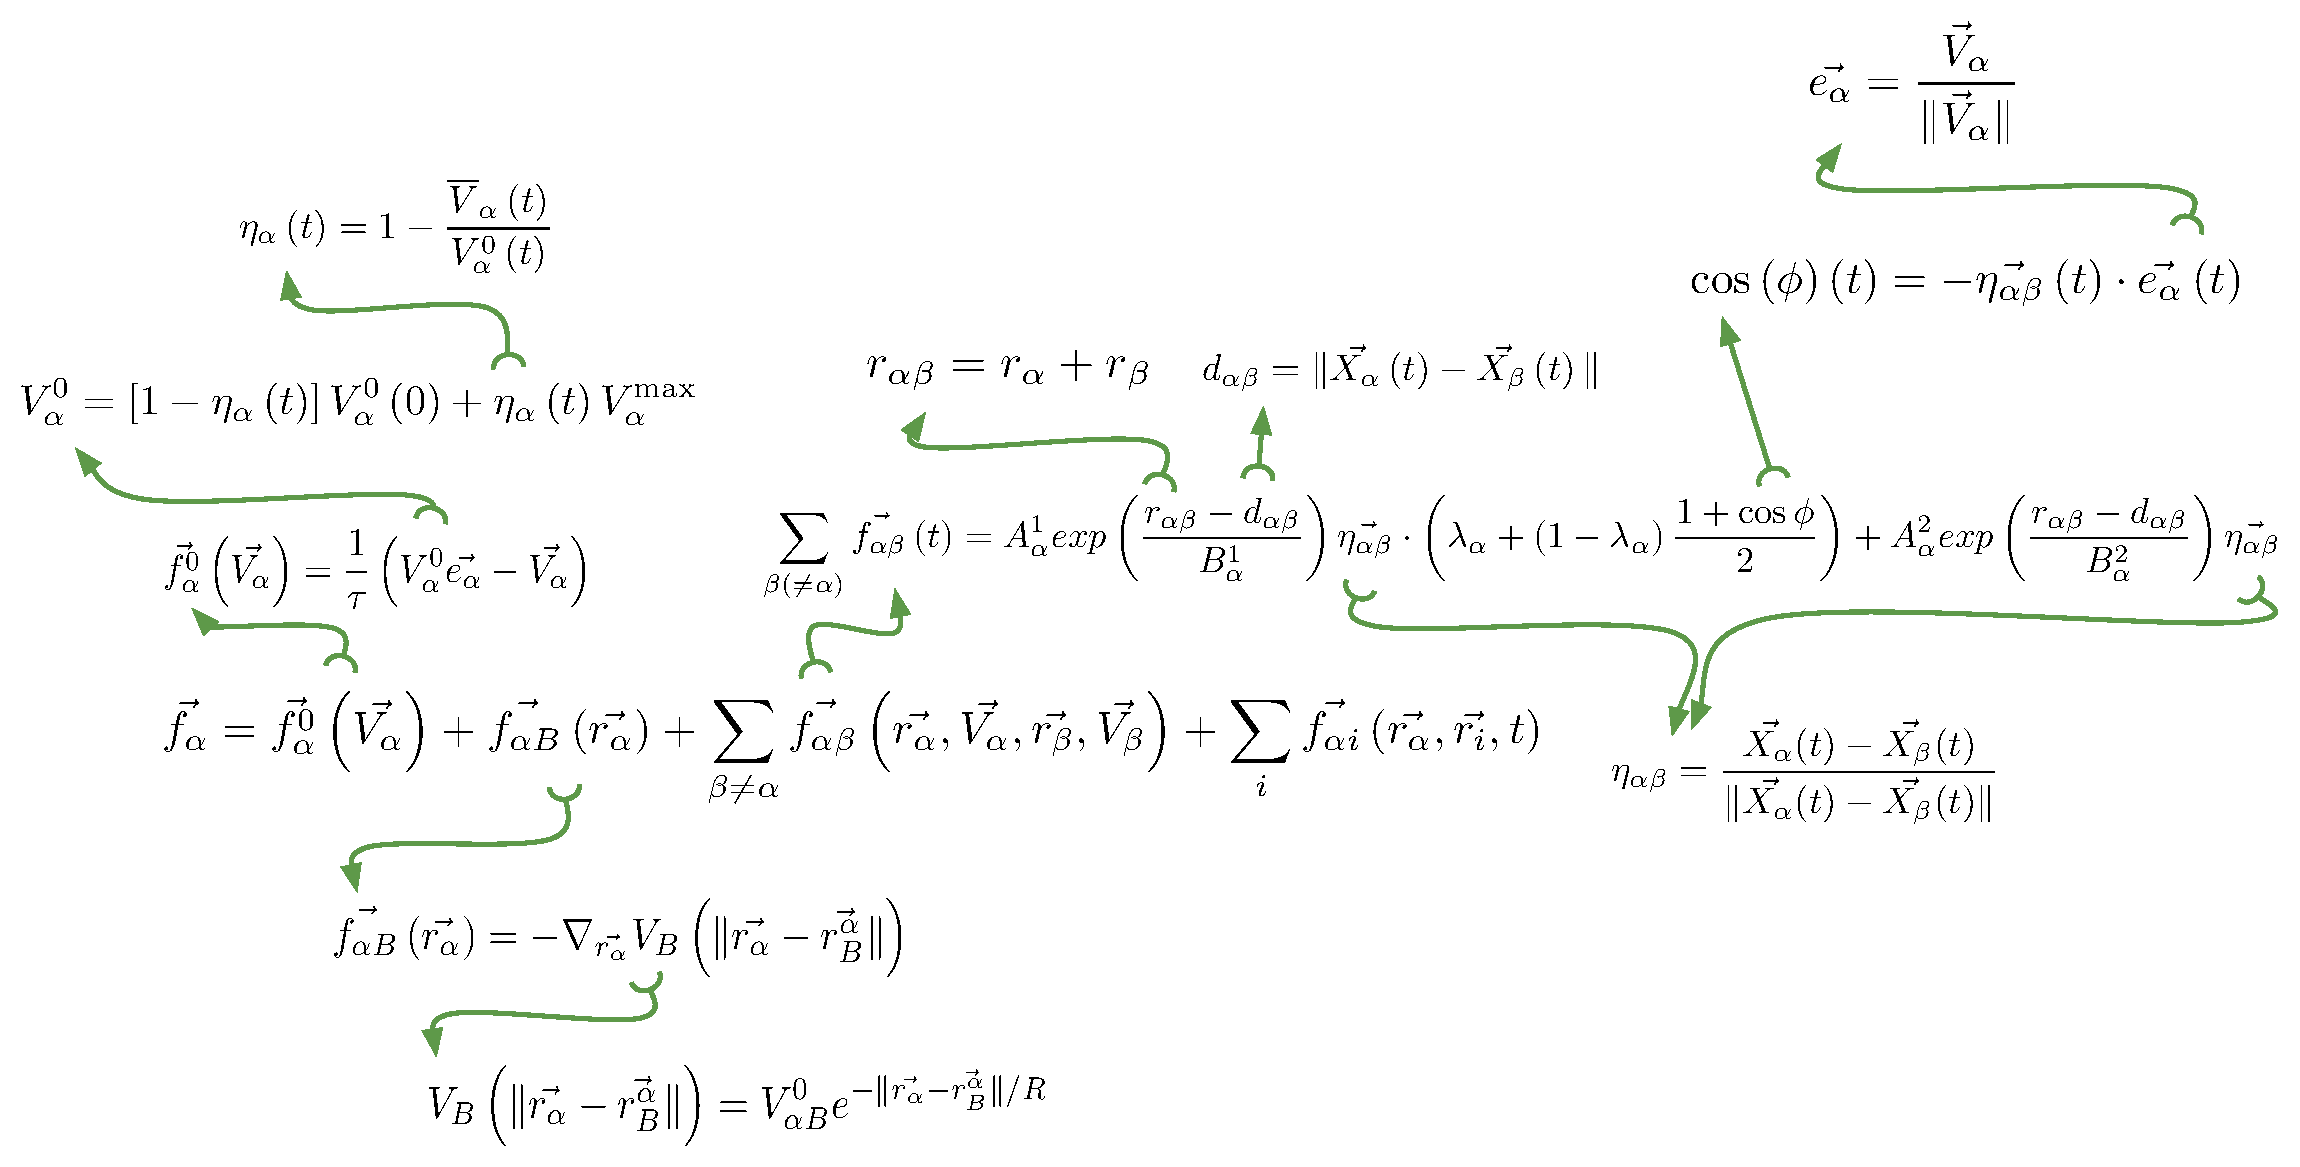
\includegraphics[scale=0.45]{Figures/overview.pdf}} 
    \caption{An overview of how the model is put together}
    \label{overview}
\end{figure}


%	I think this table should be send to the appendix							%

%	It would be nice with a figure similar to the one I (mikkel) made when i	%
%	first tried to understand the model.										%
 
\begin{center}
\begin{tabular}{lll}
\hline
\multicolumn{3}{|c|}{\emph{List of constants and variables}}\\
\hline
\small{\textbf{Symbol}} & \small{\textbf{Description}} & \small{\textbf{Unit}}\\
\hline
$A_{\alpha}^{1}$ & \small{Controls the strength of the personal space force}\\
\hline
$A_{\alpha}^{2}$ & \small{Controls the strength of physical collisions}  & \\
\hline
$B_{\alpha}^{1}$ & \small{Controls the range of the personal space force} & \\
\hline
$B_{\alpha}^{2}$ & \small{Controls the range of physical collisions} & \\
\hline
$\lambda_{\alpha}$ & The anisotropic character of pedestrian interaction & \\
\hline
$\vec{f_{\alpha}} \left( t \right)$ & All forces acting on agent $\alpha$  & \\
\hline
$\vec{f_{\alpha B}} \left( \vec{r_{\alpha}} \right)$ & Force on agent $\alpha$ from walls & \\
\hline
$\vec{f_{\alpha \beta}} \left( \vec{r_{\alpha}}, \vec{r_{\beta}}, \vec{V_{\alpha}}, \vec{V_{\beta}} \right)$ & Force on agent $\alpha$ from agent $\beta$ & \\
\hline
$\vec{f_{\alpha i}} \left( \vec{r_{\alpha}}, \vec{r_{i}}, t \right)$ & Force on agent $\alpha$ from attractions & \\
\hline
$V_{\alpha}^{0}$ & Initial speed of agent $\alpha$ & \\
\hline
$V_{\alpha}^{\text{max}}$ & Maximum speed of agent $\alpha$ & \\
\hline
$\vec{V_{\alpha}^{\text{0}}}$ & Desired velocity of agent $\alpha$ & \\
\hline
$\overline{V}_{\alpha}$ & Average speed in desired direction & \\
\hline
$\vec{e}_{\alpha}$ & Vector pointing in desired direction of agent $\alpha$ & \\
\hline
$\vec{r}_{\alpha}\left( t \right) $ & Vector pointing to position of agent $\alpha$ at time t & \\
\hline
$\vec{r}_{B}$ & Vector pointing to nearest point of wall & \\
\hline
$r_{\alpha}$ & Radius of agent $\alpha$ & \\
\hline
$r_{\beta}$ & Radius of agent $\beta$ & \\
\hline
$r_{\alpha \beta}$ & The sum of the radii of agent $\alpha$ and $\beta$ & \\
\hline
$\vec{X}_{\alpha}$ & Vector pointing to center of mass of agent $\alpha$ & \\
\hline
$\vec{X}_{\beta}$ & Vector pointing to center of mass of agent $\beta$ & \\
\hline
$d_{\alpha \beta}$ & Distance between center of mass of agent $\alpha$ and $\beta$ & \\
\hline
$\tau_{\alpha}$ & Relaxation time $\alpha$ and $\beta$ & \\
\hline
$\eta_{\alpha}$ & Impatience of agent $\alpha$ at time t & \\
\hline
$\vec{\eta}_{\alpha \beta}\left( t \right)$ & Normal vector pointing from $\alpha$ to $\beta$ at time t & \\
\hline
$\vec{\xi}\left( t \right)$ & Stochastic element & \\
\hline
$\phi_{\alpha \beta} \left( t \right)$ & Angle between agent $\alpha$ and $\beta$ & \\
\hline
\label{tableofconstandvar}
\end{tabular}
\end{center}

\clearpage
\section{sec:discussion}\label{sec:discussion}
\subsection{Repulsive force}
In chapter 3 we have seen the formulas for calculating the repulsive forces from the wall and other agents are very similar, both are exponential functions decreasing with some distance, which makes us wonder if both come from the same origin.\\

\begin{itemize}
\item The difference between those two repulsive forces is basically one is from a single point and the other is from an object that has a dimension much larger than a single agent. If we imagine our agents are particles with negative charge, then there is a pair of repulsive forces which has direction along the line connecting the two particles and magnitude depending on the distance between them. Further we can put lots of particles along a bar, see Figure
Summing up all the repulsive forces from each particle on the bar will give the repulsive force that the charged bar on the single particle $\alpha$.

\item Applying the idea above to analyse our wall repulsion, as a simple start we place the agent $\alpha$ a distance $ d $ away from the wall which as a length $L$, and by symmetry we know the resulting force must point vertically downwards, see Figure.\\

Integrating the forces can be written as:

\begin{equation}\label{integ}
\vec{f_{\alpha B}} = 
\int_0^L \! \vec{f_{\alpha\beta}} \, \mathrm{d}l
\end{equation}

\item When the repulsive force is known, the expression for the wall potential can be calculated, which can be done by integrating the force along a path. Normally the potential at some position is defined as the work done on the particle by that potential field when the particle is moved from that position to infinitely far away.

\begin{equation}\label{pot}
	U_{B}= \int_{\vec{r_{\alpha}}�}^{text{f}\infty} \! \vec{f_{\alpha B}} \cdot \, \text{d}\vec{r_{\alpha}} 
\end{equation}

\item In some article [Helbing 2000], the repulsive force from the wall is given by:
\begin{equation}\label{helbing2000}
\vec{f_{\alpha B}} = 
	\left( 
			\left[ 
	A exp 
				\left[ 
						\left(  
							r_{\alpha}-d_{\alpha B}
						\right)  / B
				\right] +kg 
					\left( 
						r_{\alpha}-d_{\alpha B} 
					\right) 
			\right] 
		\right)
	\vec{n_{B}^{\alpha}}-\kappa g 
	\left(
		r_{\alpha}-d_{\alpha B}
	\right) 
	\left(
			\vec{V_{\alpha}}\cdot \vec{t_{iw}}
	\right) 
\vec{t_{iw}}
\end{equation}

where $ r_{\alpha} $,  $ \vec{V_{\alpha}} $ are the radius and velocity of agent $ \alpha $ as we noted before, $ A $, $ B $, $ k $, $ \kappa $ are constants, $ d_{\alpha B} $ is the distance from the agent to the wall, $ \vec{n_{B}^{\alpha}} $ is a normal vector from the wall, $ \vec{t_{iw}} $ is a tangent vector to the wall. $ g $ is a function of some variable.\\
In this expression, the wall repulsion force to agent $ \alpha $ is not always perpendicular to the wall, but the force has two components, one perpendicular to the wall and the other tangent to the wall. Particularly the tangent component depends on the velocity of $ \alpha $. However, in Helbing's latest articles he does not show the expression of Equation \ref{helbing2000}, but use the gradient of potential instead. 
\end{itemize}


\subsection{The repulsive force between agents in $ \Re ^{3}$}
From the given formula for calculating the repulsive force between agents in the description of the model, the part calculating the force to keep the personal space can be omitted when the agents are rather close to each other, then the calculation can be reduced as Equation (\ref{eq:re}).

\begin{equation}\label{eq:re}
\overrightarrow{f_{\alpha\beta}}(t) = A_{\alpha}^{2} exp\left[ \frac{r_{\alpha\beta} - d_{\alpha}\beta}{B_{\alpha}^{2}}\right]  \overrightarrow{n_{\alpha\beta}}
\end{equation}

Taking the norms of both sides of Equation (\ref{eq:re}), we can draw the relation between the value of 
$\overrightarrow{f_{\alpha\beta}}(t)$ and $d_{\alpha \beta}$, as in Figure (\ref{fig:physicalinteraction})
\\
\begin{figure}
\centering
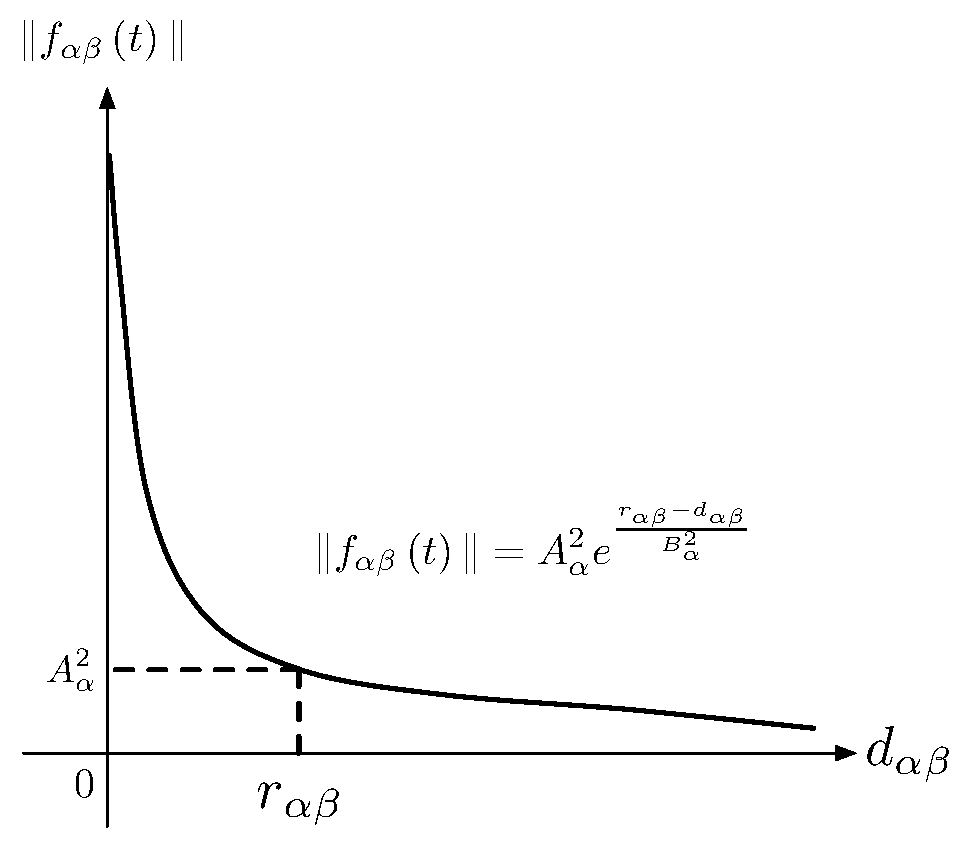
\includegraphics[scale=0.45]{Figures/physicalinteraction.pdf} 
\caption{The function about the interaction force $\vec{f_{\alpha\beta}}(t)$ and the distance between two agents
$d_{\alpha\beta}$ }\label{fig:physicalinteraction}
\end{figure}

There is one intersection of the graph and the axis $ \left( 0, A_{\alpha}^{2} exp\left( \frac{r_{\alpha\beta} }{B_{\alpha}^{2}}\right)  \right)  $. If put into the constants, we will be able to get a maximum value of $ f_{\alpha\beta}(t) $, since the distance between agents cannot be negative. Here we set $ A_{\alpha}^{2} = 3 m/s^{2} $, $ r_{\alpha\beta} = 0.6 m $, and $ B_{\alpha}^{2} = 0.2 m $, so $ f_{\alpha\beta}(t)^{max} \doteq 60 m/s^{2} $, which is about six times the gravitational acceleration and represents a rather large force between agents (as large as six person's weight). \\\\
However, we notice that the effective part of the force calculated above is only the horizontal 
component that enables the agent to move horizontally in the plane where we do the simulation, 
but the reality is that the agents sometimes are also able to move vertically, for example, 
by stepping upon other people when they cannot take the pushing force from the surrounding agents. 
When that happens, the horizontal component of the repulsive force becomes smaller even if 
$d_{\alpha\beta}$ is kept the same.	
Therefore, a qualitative modification of dependence between $ f_{\alpha\beta}(t) $ and $ d_{\alpha\beta} $ could be:
\begin{figure}[hb]   
\centering
    {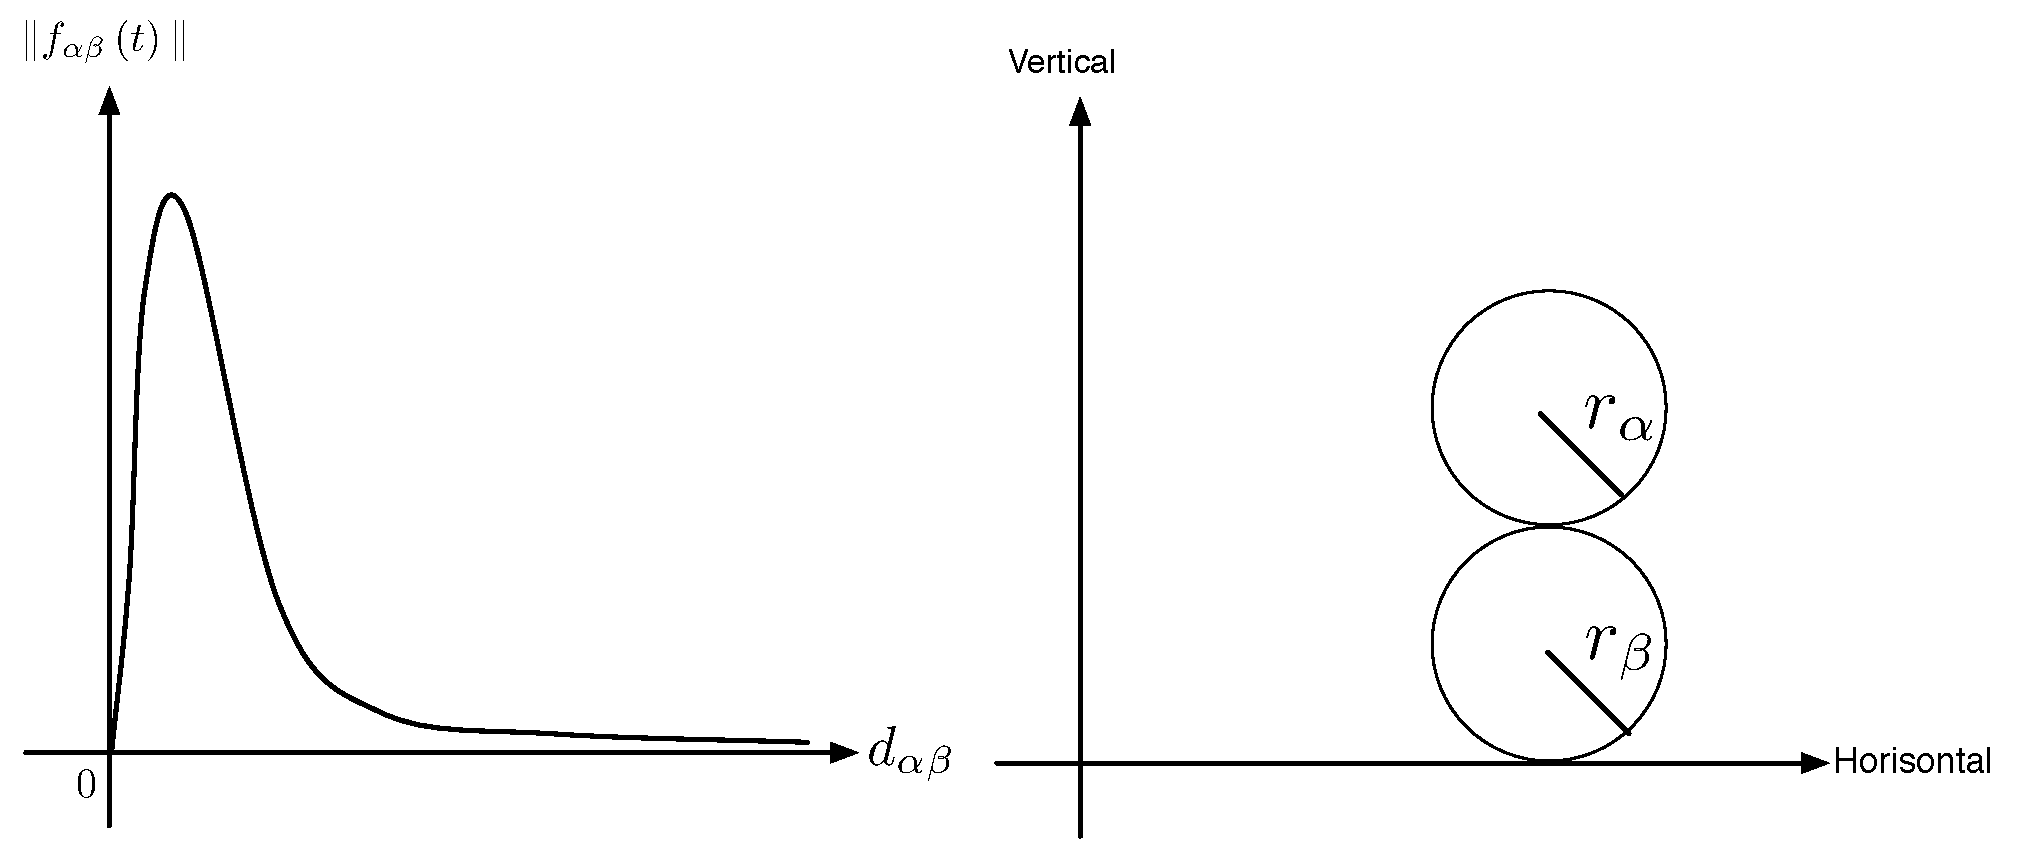
\includegraphics[scale=0.35]{Figures/ForceOverlapping.pdf}} 
    \caption{}
    \label{forceoverlapping}
\end{figure}
\\
\subsection{Use social force in further calculation}
use the value of forces to predict, as they are partly not real forces, the measurement does not reflect the reality in some range.
Pressure
